\section{Derivation of the closure terms for non-inertial dilute emulsion of spherical droplets}
\label{sec:application}

% \subsection{Discussion of the closures }



The closure presented in this section are based on the singularity solution of an isolated droplet in linear flow. 
For illustrating purposes we displayed on \ref{fig:flowlines} the flows line of such a solution both uniform flow and linear flows. 
More details on the computation of these singularity solutions are given in \ref{ap:solution_singularity}. 
Note that a quadratic background flow contribution could be taken into account since the solution is known \citep{nadim1991motion}, nevertheless it is not considered here. 
\begin{figure}[h!]
    \centering
    \begin{tikzpicture}
        % \node (img3) at (0.6\textwidth,0) {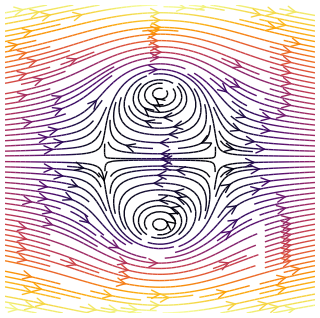
\includegraphics[width=0.3\textwidth,angle=270]{image/Rising_def_Stokes.png}};
        \node (img2) at (0.3\textwidth,0) {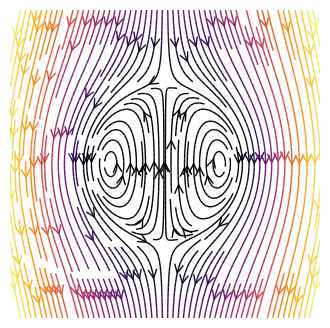
\includegraphics[width=0.3\textwidth]{image/Rising_Stokes.png}};
        % \draw (0.45\textwidth,0)node{$\rightarrow$};
        % \draw (0.45\textwidth,0.4cm)node{$\bm\Gamma_\alpha\cdot \textbf{r}$};
        \node (img1) at (0.0\textwidth,0) {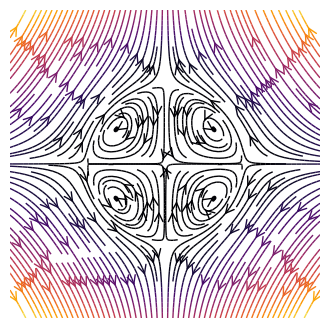
\includegraphics[width=0.3\textwidth]{image/Shear_Stokes.png}};
        % \draw (img3.south)node{(c)};
        \draw (img2.south)node{(b)};
        \draw (img1.south)node{(a)};
    \end{tikzpicture}
    \caption{Examples of steady state flow lines plots of an isolated droplet immersed into a viscous fluid. 
    (a) Rising sphere in uniform stokes flow. 
    (b) Fixed droplet in a pure extensional.
    (analytical solution in \ref{ap:solution_singularity})
    These solutions correspond exactly to the fields $\textbf{u}_f^1$ at order $\mathcal{O}(\phi_d)$.}
    % (c) Deformed droplet in rising motion (analytical solution of \citet{taylor1964deformation}). }
    \label{fig:flowlines}
\end{figure}

We recall that all along this section we consider spherical droplet of radius $a$ with viscosity ratio $\lambda = \mu_d /\mu_f$ and density ratio $\zeta =\rho_d /\rho_f$. 
Thus the problem \ref{eq:conditional_avg_eq_final_stokes} can be easily solved and have the solutions, 
\begin{align}
    \label{eq:singularity_solution_out}
    \textbf{u}_\text{out}^{1d}[\textbf{r},\textbf{w}]
    &= 
    \mathcal{U}_\text{out}[\textbf{r}] \cdot \textbf{u}
    + \mathcal{E}_\text{out}[\textbf{r}]: \textbf{E}_{f}\\
    \textbf{u}_\text{in}^{1d}[\textbf{r},\textbf{w}]
    &= 
    \mathcal{U}_\text{in}[\textbf{r}] \cdot \textbf{u}_{fw}
    + \mathcal{E}_\text{in}[\textbf{r}] : \textbf{E}_{f}
    \label{eq:singularity_solution_in}
\end{align}
where $\textbf{r} = \textbf{x} - \textbf{y}$, $\textbf{u}_{fw} = \textbf{u}_f - \textbf{w}$, the subscript ``in'' indicates that the solution is valid inside the domain $|\textbf{r}| <a$, and the subscript ``out'' in $|\textbf{r}|>a$. 
$\textbf{E}_f = \grad \textbf{u}_f + (\grad \textbf{u}_f)^\dagger$ is the shear rate tensor of the continuous phase. 
The second and third order tensor $\mathcal{U}_\text{out},\mathcal{U}_\text{in},\mathcal{E}_\text{out}$ and $\mathcal{E}_\text{in}$ read as, 
\begin{align}
    (\mathcal{U}_{\text{out}})_{ik} &= 
    \frac{1}{4}\left(\frac{3\lambda + 2}{\lambda +1}\right)
    \left(\frac{\delta_{ik}}{r} + \frac{r_ir_k}{r^3}\right) 
    + 
    \frac{1}{4}\left(\frac{\lambda}{\lambda +1}\right)
    \left(\frac{\delta_{ik}}{r^3} - \frac{3r_ir_k}{r^5}\right),  \\
    (\mathcal{E}_{\text{out}})_{ijk}
    &=
    %  \bm\delta\textbf{r}
    -\frac{\lambda}{(\lambda + 1)r^5} \bm\delta\textbf{r}
    -\left(\frac{5\lambda +2}{2(\lambda +1 )r^5} - \frac{5\lambda}{2(\lambda+1)r^7}\right) \textbf{rrr},\\
    (\mathcal{U}_{ik})_\text{in} &= 
    \frac{1}{2}\left(\frac{2\lambda +3}{\lambda +1}\right)\bm\delta
    -\frac{1}{2} (2r^2 \bm\delta - \textbf{rr})
    \left(\frac{1}{\lambda +1}\right),\\
    (\mathcal{E}_{ijk})_\text{in}
    &=
    \frac{5r^2 -3}{2(\lambda +1)} \textbf{r}\bm\delta
    - \frac{1}{\lambda+1}\textbf{rrr}. 
\end{align}


\subsection{Moment of force traction}

Let us present the closures for the momentum exchange term present in of \ref{eq:dt_hybrid_rhou_f} for dilute suspension of spherical droplets. 
% Specifically, we consider an isolated spherical non-rotating droplet of viscosity $\lambda \mu_f$ immersed in an arbitrary linear flow. 
% Most of the term present in \ref{eq:dt_hybrid_rhou_f} are discussed in\ref{ap:two-fluid_model}, thus let focus on the three exchangek terms.  
Using \ref{eq:singularity_solution_out} and \ref{eq:drag_final2} it is found that the first three moment of the hydrodynamic forces are related to the mean fluid and particle phase velocity field as, 
\begin{align}
    \label{eq:zeroth_mom}
    \pSavg{\bm{\sigma}_f^0\cdot \textbf{n}_d} &= 
    \phi_d \div\bm\Sigma_f
    + \frac{3\phi_d\mu_f}{2 a^2} 
    \left(\frac{3\lambda+2}{\lambda+1}\right) \textbf{u}_{f p} 
    + \frac{3\phi_d\mu_f}{4} \left(\frac{\lambda}{\lambda+1}\right)\grad^2\textbf{u}_f\\
    \label{eq:first_mom}
    \pavg{\intS{\textbf{r}\bm{\sigma}_f^0 \cdot \textbf{n}_d}} 
    &= 
    \phi_d \bm\Sigma_f + 
    \frac{3}{5}\mu_f \phi_d \left(\frac{2+5\lambda}{1+\lambda}\right)
    \textbf{E}_f
    \\
    \label{eq:second_mom}
        \pavg{\intS{(\bm{\sigma}_f^0 \cdot \textbf{n}_d)_ir_kr_l}} &=
        % \phi_d  \frac{a^2}{5} 3 [(\div \bm\Sigma_f)\bm\delta]^\text{sym}
        + \frac{3\mu_f\phi_d}{2}\left(\frac{\lambda}{\lambda+1}\right)(\textbf{u}_{fp})_i\delta_{kl}\\
        &+ \frac{3\mu_f\phi_d}{5}\left(\frac{1}{\lambda+1}\right)((\textbf{u}_{fp})_i\delta_{kl}+ (\textbf{u}_{fp})_k\delta_{il}+(\textbf{u}_{fp})_l\delta_{ki})\nonumber
\end{align}
where we recall that $\textbf{u}_{fp} = \textbf{u}_f - \textbf{u}_p$, $\bm\Sigma_f = -p_f\bm\delta +2 \mu_f \textbf{E}_f$, and $\textbf{E}_f = \frac{1}{2}\left[\grad \textbf{u}_f + (\grad \textbf{u}_f)^\dagger\right]$. 
Notice that at first order in $\phi_d$, $\phi_d\textbf{u}_f =\phi_d\textbf{u} - \phi_d^2 \textbf{u}_d = \phi_d\textbf{u}$, so one can either use $\textbf{u}_f$ or $\textbf{u}$ in the above definition of $\textbf{u}_{fp}$. 
The term $\pSavg{\bm{\sigma}_f^0 \cdot \textbf{n}_d}$ represents the total components of the interphase drag force.
Specifically, the first term is the mean Newtonian continuous phase stress $\bm\Sigma_f$, the second term is the Hadamard-Rybczynski force and the last is the Faxen contribution \citep{kim2013microhydrodynamics}. 
Likewise, $\pSavg{\textbf{r}\bm{\sigma}_f^0 \cdot \textbf{n}_d}$ is the averaged first moment of the surface force traction, which includes the mean fluid phase stress. 
This tensor is responsible for the well-known Einstein correction to the viscosity (see next section), but here it is adapted to spherical droplets instead of spherical solid particles \citep{rallison1978note}. 
% Therefore, this term is of upmost importance in the averaged momentum equations and is non-negligible in most of the flow conditions, if not all of them.
The second moment of the force traction is made of three contribution, the first one is related to the divergence of the mean fluid phase stress, see \ref{eq:second_mom_general}. 
However, this contribution is negligible at $\mathcal{O}(\phi_d)$ \citep{jackson1997locally} and therefor not shown in \ref{eq:second_mom}.  
The second contribution is proportional to the relative velocity $\textbf{u}_{fp}$.
This was firstly discovered by \citet{nozieres1987local} based on phenomenological arguments and by \citet{lhuillier1992volume} based on theoretical ground, both for spherical solid particles. 
According to the cited author this term induce a coupling between relative motion and convection. 
The second moment of the hydrodynamic forces is non-negligible at first order in $\phi_d$, in agreement with \citep{jackson1997locally,zhang1997momentum}. 
Thus, the zeroth, first and second moment of the drag are non-negligible in the Stokes regime and at $\mathcal(\phi_d)$. 
In \citet{zhang1997momentum} they even stipulated that the third order moment of the force traction is not necessarily negligible at $\mathcal{O}(\phi_d)$ when considering non-spherical particles in stokes flows. 

Consequently, in the stokes and dilute hypothesis, the zeroth, first and third moments of surface traction are non-negligible and are primordial in the modeling of the fluid phase momentum equations. 
It is therefore reasonable that these terms are also relevant for broader flows regime. 
For example, in \ref{chap:deformable} we demonstrate that \ref{eq:first_mom} has a component proportional to the mean phase velocity $\textbf{u}_{fp}\textbf{u}_{fp}$ in the inertial regime. 
Thus, it is surprising that most studies in the literature do not mention the first and second-order moments, which are almost always neglected

\subsection{Pseudo turbulent stress}

Another contribution to the stress is the pseudo-turbulent tensor $\avg{\chi_f \textbf{u}_f'\textbf{u}_f'}$. 
Note that in stokes regime this term is more likely to be negligible, nevertheless it is still interesting to provide its closure based on the Stokes solution as it gives the first order inertial contribution, which is of course non-negligible at finite particle Reynolds number.

In \ref{ap:solution_singularity} we compute this closure based on \ref{eq:Batchelor2}, following the rigorous methodology presented in the previous section.  
In brief the methodology is as follows:
According to \ref{eq:Batchelor2} we may reformulate $\avg{\chi_f \textbf{u}_f'\textbf{u}_f'}$ in terms of an integral of $\textbf{u}_\text{out}^{1d}\textbf{u}_\text{out}^{1d}$ over all the particle velocity $\textbf{w}$ and position $\textbf{y}$. 
In the Stokes regime $\textbf{u}_\text{out}^{1d}$ is proportional to $\textbf{u}_{fw} = \textbf{u}_f - \textbf{w}$ and $\textbf{E}_f$, see \ref{eq:singularity_solution_out}. 
Since, $\avg{\chi_f \textbf{u}_f'\textbf{u}_f'}$ is a symmetric second order tensor, the final closure must remain symmetric and second order.
Additionally, the only possible combination of tensor, $\textbf{u}_{fw}$ and $\textbf{E}_f$, which can form a symmetric second order tensor are, 
\begin{align}
    \textbf{u}_{fw}
    \textbf{u}_{fw}
    &&
    \textbf{E}_f\cdot \textbf{E}_f
    && 
    (\textbf{u}_{fw}\cdot 
    \textbf{u}_{fw})\bm\delta
    &&
    (\textbf{E}_f : \textbf{E}_f)\bm\delta. 
\end{align}
Notice that it is impossible to obtain a second order tensor based on combination of one vector ($\textbf{u}_{fw}$), and one second-order tensor ($\textbf{E}_f$). 
Therefore, we deduce that at the leading order in Reynolds number and particle volume fraction no correlation exist between the wake of a particle in translation and its distance field in shearing motion. 
Note that at higher Reynolds number we might found terms proportional to $Re \textbf{u}_{fw}\textbf{u}_{fw} \cdot \textbf{E}_f$. 

We conclude that the functional form of $\avg{\chi_f \rho_f \textbf{u}_f' \textbf{u}_f'}$ must be of the form, 
\begin{multline}
     \avg{\chi_f \rho_f \textbf{u}_f' \textbf{u}_f'}
     =
     C_{uu}^1 [\textbf{u}_{fp} \textbf{u}_{fp}+ \pavg{\textbf{u}_\alpha' \textbf{u}_\alpha'}]
     + C_{EE}^1 \textbf{E}_f\cdot \textbf{E}_f \\
     + \left[ 
         C_{uu}^2 (\textbf{u}_{fp}\cdot  \textbf{u}_{fp} + 2k_p)
         +  C_{EE}^2 (\textbf{E}_f : \textbf{E}_f)
    \right]\bm\delta
    \label{eq:Reynolds_stress_functional_form}
\end{multline}
where $C_{uu}^1,C_{EE}^1,C_{uu}^2$ and $C_{EE}^2$ are yet unknown scalar function. 
Note that the particle center of mass velocity variance $\pavg{\textbf{u}_\alpha' \textbf{u}_\alpha'}$ and $2k_p = \pavg{\textbf{u}_\alpha' \cdot \textbf{u}_\alpha'}$ are present in \ref{eq:Reynolds_stress_functional_form} because, 
\begin{equation}
    n_p[\textbf{x},t]\int_{\mathbb{R}^3} \textbf{u}_{fw}\textbf{u}_{fw} P[\textbf{w}|\textbf{x},t] d\textbf{w}
    =  
    \avg{\textbf{u}_\alpha'\textbf{u}_\alpha'}. 
\end{equation}
Physically \ref{eq:Reynolds_stress_functional_form} means that each droplet in a flow, induces pseudo turbulence through their relative linear motion $\textbf{u}_{fw}$, i.e. which is exactly the wake on \ref{fig:flowlines} (left), and the wake when mean linear motions acts around the droplets, see  \ref{fig:flowlines} (right). 
Note also that the terms on the second line represent the isotropic part of the Reynolds stress tensor,  which is $3/2$ of the pseudo-turbulent energy: $k_f$. 


The disturbance fields of a droplet in translation is proportional to $r^{-1}$ (see \ref{eq:singularity_solution_out}) thus the computation of the integral of $\avg{\chi_f \rho_f \textbf{u}_f' \textbf{u}_f'}$ in the case of translation diverges if we use \ref{eq:Batchelor2}.
This divergence issue is well known in fluid mechanics \citep{caflisch1985variance}, therefore at this stage we are unable to compute the coefficient $C_{uu}^1$ and $C_{uu}^2$ that are related to translational motions. 
As mentioned in the previous section, (see also \ref{chap:pseudoturbulence}), this divergence issue arise because \ref{eq:Batchelor2} is unable to provide physical results in this regime. 
Nevertheless, as stated above the functional form of this tensor cannot be otherwise that proportional to $\textbf{u}_{fw} \textbf{u}_{fw}$ and $(\textbf{u}_{fw}\cdot \textbf{u}_{fw})\bm\delta$.
To support that hypothesis, note that when only considering the translational motion ($\textbf{E}_f = 0$), for spherical bubbles in potential flow, the pseudo turbulent tensor have the same functional form as \ref{eq:Reynolds_stress_functional_form} (see equation (5.7) of \citet{zhang1994ensemble}). 
Additionally, for ordered array of spheres immersed in a uniform non-inertial flow we found that $C_{uu}(\phi) \sim \phi^{2/3}$ \citet{hill2001first}.
It is therefore reasonable to expect the same trend for random array.
In \ref{chap:pseudoturbulence} we provide a novel strategy to compute $C_{uu}^1$ and $C_{uu}^2$ based on a different statistical framework. 


The contribution from the mean shear flow $\textbf{E}_f$ to the pseudo turbulent tensor is derived in \ref{ap:solution_singularity} based on \ref{eq:Batchelor2}, which works fine in this case. 
Indeed, as the wake of a particle in pure linear flow decay as $\mathcal{O}(r^{-3})$ the error in \ref{eq:Batchelor2} remains finite providing physical results. 
Carrying out the integration we directly obtain, 
\begin{align*}
    C_E^1  = \frac{\phi_d a^2 \rho_f}{105 (\lambda +1)^2 } (129\lambda^2+108\lambda+24)\\
    C_E^2 = \frac{\phi_d a^2 \rho_f}{105 (\lambda +1)^2 } (20\lambda^2 +20\lambda + 6)
\end{align*}
In  \citet{raja2010inertial} they study theoretically the stress in a neutrally buoyant suspensions of droplets. 
In the dilute limit they compute the deviatoric part of $\avg{\chi_f \rho_f \textbf{u}_f' \textbf{u}_f'}$ based on the stokes flow solution. 
It is observed that $C_E^1$ is consistent with equation (3.15) of \citet{raja2010inertial}.
Regarding $C_E^2$ it corresponds to the  isotropic contribution of the Reynolds stress.
To the knowledge of the author this result has never been presented in the literature.


\subsection{The fluid phase equivalent stress}
% In this section we focus on the formulation of the averaged fluid phase equivalent stress tensor $\bm{\sigma}_f^\text{Re}$. 
For instance the stress appearing on the left hands side of the fluid phase momentum balance is of the form of \ref{eq:sigma_eq_def}. 
It is more convenient to express the equivalent stress as a Newtonian stress, plus a contribution arising due to the presence of the particles. 
Thus, we reformulate $\bm{\sigma}_f$ considering that $\phi_f \bm{\sigma}_f = - \phi_f p_f + 2 \phi_f \mu_f \textbf{e}_f$ where $2 \phi_f \bm{e}_f = \avg{\chi_f  (\grad \textbf{u}_f^0 + (\grad \textbf{u}_f^0)^T)}$. 
Additionally, we state that the fluid strain is equal to the bulk strain $2\textbf{e} = \grad \textbf{u}+ (\grad \textbf{u})^T$, minus the particle averaged strain, i.e. $\phi_f \mu_f \textbf{e}_f = \mu_f\textbf{e} - \mu_f \phi_d \textbf{e}_d$ which gives
\begin{equation*}
    \bm\sigma_f\phi_f =-\phi_f p_f \bm\delta + 2 \mu_f \textbf{e} -2\phi_d \mu_f \textbf{e}_d.
    \label{eq:def_sigma_f}
\end{equation*}
Under this form we clearly remark that for solid particle $\phi_d \textbf{e}_d = 0$ thus we recover equations (44) of \citet{jackson1997locally} which reads in our notation : $\bm\sigma_f\phi_f =-\phi_f p_f \bm\delta + 2 \mu_f \textbf{e}$. 
Upon developing $\phi_d \textbf{e}_d$ multipolar series using \ref{eq:f_exp}, the equivalent stress of the fluid phase can be reformulated as, 
\begin{multline}
    \bm{\sigma}^\text{eq}_f = 
    \phi_f p_f \bm\delta 
    - 2\mu_f \textbf{e} 
    +\avg{\rho_f\chi_f\textbf{u}_f'\textbf{u}_f'} 
    + 2 \mu_f \pOavg{\textbf{e}_d^0}
    - \pSavg{\textbf{r}\bm{\sigma}_f^0\cdot \textbf{n}_d}
    \\
    + \div \left[
        \frac{1}{2} \pSavg{\textbf{rr}\bm{\sigma}_f^0\cdot \textbf{n}_d}
        - 2 \mu_f\pOavg{ \textbf{re}_d^0 }
        + \ldots
    \right]
    \label{eq:sigma_eq_0}
\end{multline} 
It is worth noting that $\textbf{e} = \grad \textbf{u} + (\grad \textbf{u})^\dagger$. 
Nevertheless, the bulk velocity \textbf{u} is not part of our unknown in the ``hybrid model'', instead we solve for $\textbf{u}_f$, $\textbf{u}_p$, $\textbf{P}_p$ and eventually the higher moments. 
Therefore, in all rigor we must write 
\begin{equation}
    \textbf{e}
    = 
    \textbf{E}
    - \grad (\div (n_p \textbf{P}_p))
    - (\grad \div (n_p \textbf{P}_p))^\dagger
    + \ldots
    \label{eq:rate_of_strain}
\end{equation}
where $\textbf{E} = \grad \textbf{U} + (\grad \textbf{U})^\dagger$ with $\textbf{U} = \phi_f \textbf{u}_f + n_p v_p \textbf{u}_p$ is equivalent to the bulk velocity \textbf{u} uniquely in an homogeneous medium. 

% The fluid phase averaged stress is therefore composed of : 
% (1) the pseudo turbulent contribution $\rho_f\avg{\chi_f  \textbf{u}_f' \textbf{u}_f'}$ which can be decomposed in an isotropic part $2 k_f = \avg{\chi_f \rho_f \textbf{u}_f' \textbf{u}_f'}:\bm\delta$ that contribute to the effective pressure, and a deviatoric part defined as $\avg{\chi_f \rho_f \textbf{u}_f' \textbf{u}_f'} - 2 k_f\bm\delta$. 
% (2) the shear stress $2\mu_f \textbf{e}$ of the fluid phase \ref{eq:rate_of_strain}. 
% (3) the particles internal shear $2\mu_f \pOavg{\textbf{e}_d^0}$
% (4) the particle first moment of the hydrodynamic forces $\pSavg{\textbf{r}\bm{\sigma}_f^0\cdot \textbf{n}_d}$. 
% (5) and the higher order moments of forces and internal shear.  

At this point if one want to write the fluid phase averaged stress as an equivalent Newtonian stress with effective pressure $p^{eff}$ and effective viscosity $\mu^{eff}$ he needs to express each of the closure terms mentioned above as a function of an isotropic tensor which will contribute to the effective pressure, or as a linear function of  $\textbf{e}$ which will contribute to the effective viscosity. 
Note that this is not always possible, indeed, according to \ref{eq:second_mom} the second order moment of the hydrodynamic stress is a function of the relative velocity and not of the mean shear rate. 
Thus, in addition to the Newtonian behavior of the averaged fluid one must be prepared to find non-Newtonian terms purely related to the dispersed nature of the flow. 

To that end we compute the fourth last terms on the right-hand side of \ref{eq:sigma_eq_0} and find (see \ref{ap:solution_singularity}), 
% \begin{align}
%     \pOavg{\textbf{e}_d^0}
%     = 
%     \phi_d 
%     \textbf{E}_f
%     \frac{3}{5}\frac{1}{\lambda+1}
%     \\
%     \pOavg{\mu_f \textbf{e}_d^0\textbf{r} }
%     = 
%     - \frac{\phi_d\mu_f}{10(\lambda+1)}
%     \left[
%         (\bm\delta \textbf{u}_{fp})_{ijk}
%         - \frac{3}{2}
%         \left[
%             (\bm\delta \textbf{u}_{fp})_{kij}
%             + (\bm\delta \textbf{u}_{fp})_{jki}
%         \right]
%     \right]
%     \label{eq:closur_e}
% \end{align}
% Notice that the second moment of momentum is present under the $\partial_k\partial_l$ operator in the moment of momentum equation, meaning that the skew-symmetic part of $\pavg{\intS{(\bm{\sigma}_f^0 \cdot \textbf{n}_d)_ir_kr_l}} $ and $\pSavg{{\mu(\textbf{e}_d^0)_{ik} r_l}}$ vanish in the momentum equation. 
% Therefore, the second moment of surface traction force might be written, 
\begin{align*}
    \pavg{\intS{(\bm{\sigma}_f^0 \cdot \textbf{n}_d)_ir_k}} -
    2\pSavg{{\mu(\textbf{e}_d^0)_{ik}}} 
    &= 
    \phi_d p_f\bm\delta
    - \frac{5\lambda +2}{\lambda +1}
    \textbf{E}_f \phi \mu_f
    \\
    \frac{1}{2}\pavg{\intS{(\bm{\sigma}_f^0 \cdot \textbf{n}_d)_ir_kr_l}} -
    2\pSavg{{\mu(\textbf{e}_d^0)_{ik} r_l}} 
    &= 
    \frac{\mu_f\phi_d}{2(\lambda +1) }
    \left[
        \frac{3\lambda}{2} 
        u_{fp,i}\delta_{kl}
        +  u_{fp,l}\delta_{ki}
    \right]. 
\end{align*}
Considering this relation together with \ref{eq:sigma_eq_0} we can re-write the effective stress of the suspension as, 
\begin{multline}
    \bm{\sigma}^\text{eq}_{f,ik} =
    + \rho_f\avg{\chi_f\textbf{u}_f'\textbf{u}_f'}_{ik} 
    + p_f \bm\delta
    - 2 \mu_f \textbf{E}\left[
        1
        +\frac{\phi_d}{2}\left(
            \frac{5\lambda +2}{\lambda +1}
        \right)
    \right]\\
    + 
    \frac{\mu_f 3\lambda}{4(\lambda +1) }
    \left[
        \grad (\phi_d\textbf{u}_{fp,i})
        +  
        \frac{2}{3\lambda} 
        [\div (\phi_d\textbf{u}_{fp,l})]\bm\delta_{ki}
    \right]
\end{multline} 
where the \textit{Reynolds stress} tensor is given by \ref{eq:Reynolds_stress_functional_form}, in which $C_E^1$ and $C_E^2 = \mathcal{O}(Re)$ and are therefore negligible compared to the first moment, while $C_{uu}^1$ and $C_{uu}^2$ are still unknown constant. 
This expression is in agreement with \citet[Appendix A]{zhang1997momentum}. 
In order to highlight that the stress tensor is symmetric we add and remove the term $ \grad \textbf{u}_{fp,i}^\dagger$  to the stress and notice that only the symmetric part in the indices $kl$ remain under the application of the double gradient operator present in the momentum equation. 
Based on similar arguments than \ref{eq:sym_proof} we can show that it gives, 
\begin{multline}
    \bm{\sigma}^\text{eq}_{f,ik} =
    + \rho_f\avg{\chi_f\textbf{u}_f'\textbf{u}_f'}_{ik} 
    + p_f \bm\delta
    - 2\mu^\text{eff} \textbf{E}
    + \\
    \mu_\text{U}^\text{eff}
    \left[
        \partial_k   (\phi_d\textbf{u}_{fp,i})
        + \partial_i (\phi_d\textbf{u}_{fp,k})
        + \frac{2-3\lambda}{3\lambda}  [\div (\phi_d\textbf{u}_{fp,l})]\bm\delta_{ki}
    \right]
    \label{eq:fluid_phase_stress}
\end{multline} 
Where the equivalent viscosity of the fluid are given by 
\begin{align*}
    \mu^\text{eff} = \mu_f \left[
        1
        +\frac{\phi_d}{2}\left(
            \frac{5\lambda +2}{\lambda +1}
        \right)
    \right] &&
    \mu^\text{eff}_\text{U}
    = \mu_f\frac{ 3\lambda}{4(\lambda +1) }
\end{align*}
We conclude that, neglecting the terms of $\mathcal{O}(Re,\phi^2_d)$, and considering that $\textbf{u}_f$ is purely linear at the scale of the particle, the equivalent stress is not Newtonian since it has an additional contribution arising from the relative phase velocity appears. 


\subsection{Energy exchange terms}

The energy exchange terms in \ref{eq:dt_hybrid_rhoE_f} and \ref{eq:dt_hybrid_Ep} come either from a heat source or form mechanical work. 
As the former contribution is not treated in this study we rather focus on the mechanical work exchange terms. 
Thus, let us focus in the first place on the last term of \ref{eq:exergysource}.

As mentioned above this term represents the source of pseudo turbulent energy in the fluid phase due to the work done locally on the surface of the particle through the local velocity $\textbf{w}_d^0$ and the local stresses $(\bm\sigma_f^0 \cdot \textbf{n})$.
Reformulating this term in terms of \textit{single-particle} conditionally average velocity field, leads us to, 
\begin{equation}
    \pavg{ \intS{\textbf{w}_d^0 \cdot \bm{\sigma}_f^0 \cdot \textbf{n}_d}}
    \approx
    \int_{\mathbb{R}^3} \int_{|\textbf{r}| = a}
    [(\textbf{u}^1_f - \textbf{w})\cdot \bm\sigma_f^1\cdot \textbf{n} ]
    d\textbf{r}
    P_1[\textbf{x},\textbf{w}]
    d\textbf{w} 
    \label{eq:reformulation_wsigma_n}
\end{equation} 
Notice that this is only an approximation, since in all rigor, a correlation term appear due to the ensemble average of the product $\textbf{w}_d^0 \cdot \bm{\sigma}_f^0$ transformed in product of averaged terms. 
However, going into deeper complexity is out of the context of this work.  
The velocity field in \ref{eq:reformulation_wsigma_n} can be obtained directly from \ref{eq:singularity_solution_in}  evaluated at the surface of the particle test, thus we can write that,
\begin{equation*}
    \textbf{u}^1_f - \textbf{w}
    = 
    \frac{1}{\lambda +1} \left[\left(
        -\frac{\bm\delta}{2}
        + 
        \frac{\textbf{rr}}{2a^2}
    \right)\cdot (\textbf{u}_{f} - \textbf{u}_\alpha) 
    + \left(\textbf{r}\bm\delta
    -\frac{1}{a^2}\textbf{rrr}\right)\cdot \textbf{E}_f
    \right].
\end{equation*}
Note that this fields is a combination of the fields displayed in \ref{fig:flowlines} (left) and (right), evaluated at the surface of the droplets. 
The contributions of the velocity field factor of $\textbf{u}_{fp}$ represents the famous hill's vortex reticulation inside a spherical droplet. 
The second contribution is the motion at the surface of the droplet generated due to a mean shear flow. 

Injecting this expression into \ref{eq:reformulation_wsigma_n} gives, 
\begin{align}
    &\pSavg{\textbf{w}_2^0 \cdot \bm{\sigma}_1^0\cdot\textbf{n}_2}
    =  \\
    &\frac{1}{\lambda+1}\textbf{u}_{fp} \cdot \left[
        -\frac{1}{2}\pSavg{ \bm{\sigma}_1^0\cdot\textbf{n}_2}
        % + \pavg{\textbf{u}_{\alpha}' \cdot \intS{ \bm{\sigma}_1^0\cdot\textbf{n}_2} }
        + \frac{1}{2a^2}
        \pSavg{\textbf{rr}\cdot \bm{\sigma}_1^0\cdot\textbf{n}_2}
    \right]\nonumber
    \\
    &+ \frac{1}{\lambda+1} \left[
        -\frac{1}{2}
        \pavg{\textbf{u}_\alpha' \cdot  \intS{\bm{\sigma}_1^0\cdot\textbf{n}_2}}
        % + \pavg{\textbf{u}_{\alpha}' \cdot \intS{ \bm{\sigma}_1^0\cdot\textbf{n}_2} }
        + \frac{1}{2a^2}
        \pavg{\textbf{u}_\alpha' \cdot \intS{\textbf{rr}\cdot \bm{\sigma}_1^0\cdot\textbf{n}_2}}
    \right] \nonumber
    \\
    % \left[
    %     \textbf{u}_{p f} \cdot
    %     +
        % \pavg{\textbf{u}_{\alpha}' \cdot \intS{\textbf{rr}\cdot \bm{\sigma}_1^0\cdot\textbf{n}_2}}
    % \right]
    &+ \frac{1}{\lambda + 1} \textbf{E}_{f} : \left[ 
         \pSavg{\textbf{r} \bm{\sigma}_1^0\cdot\textbf{n}_2}
         -\frac{1}{a^2} 
         \pSavg{ \textbf{rrr} \cdot \bm{\sigma}_1^0\cdot\textbf{n}_2}
         \right]
    \label{eq:energy_term}
\end{align}
% \tb{maybe explicite those terms and disscus and compare with L. M. Liljegren (1996) for solid particles; say that he neglect all of the first moments }
In this expression we clearly identify the zero, first and second order moments of the surface force traction provided by \ref{eq:first_mom}. 
Additionally, notice that we did not consider rotation of droplets consequently the mean fluid vorticity nor the particles angular velocity appears in this expression. 
One can also notice that taking the limit $\lambda \to \infty$ gives zero for \ref{eq:energy_term}. 
Which is consistent since $\textbf{w}_d^0 = 0$ for non-rotating solid particles. 
Consequently, in light of \ref{eq:energy_term} the work generated due to the local motion at the surface of a spherical droplet, namely  $\pSavg{\textbf{w}_2^0 \cdot \bm{\sigma}_1^0\cdot\textbf{n}_2}$ is either due to its relative motion with the continuous phase  or due to its simple presence in a shear flow. 
Indeed, in both cases motion at the surface of the particle is observed and stresses is also generated, which in turns contribute the generation of pseudo turbulence. 
In fact if we add the contribution given by \ref{eq:energy_term} in  \ref{eq:dt_hybrid_k1} we observe that  the consideration of hill's vortexes add the coefficient $\frac{\lambda +\frac{1}{2}}{\lambda+1}$ in front of the drag force velocity terms in \ref{eq:dt_hybrid_k1}.
Besides, the first moments of surface traction forces appearing in the diffusive equivalent flux $\textbf{q}_1^k$ are also subject to these comments.  
Consequently, the consideration of hill's vortex end up to add a coefficient in front of this exchange term which varies from $1$ to $1/2$ for respectively, solid particles and bubbles.  
Same comments can be made regarding the consideration of the droplets internal motion to the higher moments present in the flux term $\textbf{q}^k_f$. 

As a matter of fact the consideration of the internal motion of particles such as hill's vortex have a very significant impact regarding the magnitude of the pseudo turbulent exchange terms, especially when one is considering bubbly flow. 
The physical explanation of the decrease of the coefficient in front of the exchange terms for bubbles, can be due to the facts that the fluid slip on the bubbles or droplet's surface induce less work exchange than if the fluid followed the particle's surface as it is the case for solid particles. 

In the literature it is customary to use a ``Modulation parameter'' that account for the fact that not all the kinetic energy is transmitted form the dispersed to the continuous phase due to slip at the bubbles surfaces of the particles.
Specifically this parameter ``that controls the fraction of interfacial turbulence transferred.'' \citep{magolan2019quantitative}. 
Even, if there is no direct equivalence between the ``Modulation parameter'' and the above analysis we may argue that the latter is partly driven by the slip velocity at the interface. 
While many empirical models have been proposed (see Table 1 of \citet{magolan2019quantitative}) it seems that none of them make use of theoretical arguments as it is presented here.
However, our ``Modulation parameter'' is of $1/2$ for bubbles while the empirical studies shown that it should be $0.25$, which is quite close.


\subsection{Particles induced dissipation in the continuous phase}

Another closure of upmost importance in the pseudo turbulent equation is the fluid phase dissipation $\avg{\chi_f \bm\sigma_f^0 :\grad\textbf{u}_f^0}$. 
Here we propose to compute this term based on  methodology presented in \ref{ap:Closure_problem}. 
Thus, we only consider, what we call the \textit{particle induced dissipation} and not the dissipation due to single-phase turbulence for example.
This means that we consider only the dissipation in the fluid phase that is due to particle relative motions. 
Using the same methodology as for the \textit{Reynolds stress} closure, we find using \ref{eq:singularity_solution_out} the following expression: 
\begin{multline}
    \avg{\chi_f \bm\sigma_f^0 :\grad\textbf{u}_f^0}
    =
    \frac{3\mu_f \phi_d}{2a^2}
    \frac{(3\lambda^2 + 4\lambda +2)}{(\lambda + 1)^2}
    (\textbf{u}_{fp}\cdot \textbf{u}_{fp} + 2 k_p ) \\
    + 
    \frac{3\mu_f \phi_d}{5}
    \frac{(5\lambda^2 + 4\lambda +4)}{(\lambda + 1)^2}
    \textbf{E}_f:\textbf{E}_f
    +2 \phi_f \textbf{E}_f:\textbf{E}_f
    \label{eq:dissipation_term}
\end{multline}
We can observe that the first two terms are related to the particle relative translation with the continuous phase. 
The second term is the contribution to the fluid phase dissipation due to the  disturbance field of particle in linear flow. 
As for the Reynolds stress, notice that the terms of the for $\textbf{u}_{pf}$ times $\textbf{E}_f$ are not present in this equation since it is impossible to form a scalar which is linear with a vector and a second order tensor. 



The remaining closures in the equation of $k_p$, i.e. $\rho_f \avg{\chi_f \textbf{u}_f' k_f}$ and $\avg{\chi_f \textbf{u}_f' \cdot \bm{\sigma}_f^0}$, are in fact null in stokes flow. 
This is because these terms are by nature produced due to the asymmetry of the disturbance fields. 

To the authors' knowledge this closure \eqref{eq:dissipation_term} is original and must be used as a theoretical ground to develop more sophisticated closure for the dissipation term in multiphase flow.

\subsection{Particles internal kinetic energy and dissipation}
% Most of the closure terms present in these expressions also appear in the continuous phase. 
% They have therefore already been discussed. 
Now we discuss the term appearing on the right-hand side of \ref{eq:dt_hybrid_Wp} which appears only in the particle-phase equations. 
Based on the velocity field given by \ref{eq:singularity_solution_in} we might compute directly the following closures,
\begin{align}
    \label{eq:stokes_Wp}
    W_p =  \frac{\rho_d \phi_d}{24 (\lambda +1)^2}
    (\textbf{u}_{fp} \cdot \textbf{u}_{fp} + 2 k_p)
    + \frac{a^2 \rho_d \phi_d}{30(\lambda+1)^2}
    \textbf{E}_f:\textbf{E}_f    \\
    \pOavg{\bm{\sigma}_2^0:\grad \textbf{u}_2^0}
    % = 2\mu_2 \intO{\textbf{e}_2^0: \textbf{e}_2^0 }
    = 
    \frac{6 \phi_d \mu_f \lambda}{a^2(1+\lambda)^2}
    (\textbf{u}_{fp}\cdot \textbf{u}_{fp} + 2k_p)
    + \frac{3 \phi_d \mu_f \lambda}{(\lambda+1)^2}\textbf{E}_f:\textbf{E}_f
    \label{eq:diff_d}
\end{align}
From \ref{eq:stokes_Wp} we deduce that the relative motion between phases $\textbf{u}_{pf}$, as well as the mean gradient of the flow $\textbf{E}_f$ induce an inner kinetic energy inside the droplet. 
The dissipation term given by \ref{eq:diff_d} represents the energy dissipated into heat inside the particles. 
Since the motion inside the particles is directly determined by $\textbf{u}_{pf}$ and $\textbf{E}_f$ the dissipation rate within it is equally. 
Thus, this term directly witness of the heat induced within the particle directly due from mean phase motion. 

\subsection{Second moment equations closure}

The second moments equations describe the shape and the rate of deformation of the particles.
In this section we assumed implicitly that the droplets remain spherical due to the low capillary number considered. 
Therefore, \ref{eq:dt_hybrid_Mp} and the deviatoric part of \ref{eq:dt_hybrid_Sp} is of no use. 
Moreover, we didn't consider rotation of the particles as well, thus \ref{eq:dt_hybrid_mup} cannot be discussed further. 
Nevertheless, computing the closure terms present in of these equations for spherical droplets still gives us hints of their physical significance that will have when we will consider deformation in \ref{chap:deformable}. 
Therefore, for pedagogical purposes we now discuss the terms present in \ref{eq:dt_hybrid_Sp} for droplets in an arbitrary linear flow. 


% Because of \ref{eq:eq:Batchelor}, a droplet in an arbitrary linear stokes flow remains spherical at low capillary number due to the competitive contribution of the drop internal stress, the interfacial stress and the surface tension, namely, 
% \begin{align*}
%     \intO{\bm{\sigma}_d^0},
%     &&\frac{1}{2}\intS{(\textbf{r}\bm\sigma_f^0+\bm\sigma_f^0\textbf{r})\cdot \textbf{n}},
%     &&\intS{\gamma(\bm\delta - \textbf{nn})},
% \end{align*}
% respectively. 

From  \ref{eq:Batchelor} we deduce that in the Stokes regime, 
\begin{equation*}
    \pSavg{\gamma(\bm\delta - \textbf{nn})}
    = 
    \frac{1}{2}\pSavg{(\textbf{r}\bm\sigma_f^0+\bm\sigma_f^0\textbf{r})\cdot \textbf{n}}
    - \pOavg{\bm{\sigma}_d^0},
\end{equation*}
Thus, a droplet in an arbitrary linear stokes flow remains spherical at low capillary number due to the competitive contribution of the drop internal stress, the interfacial stress and the surface tension
The contribution from the continuous phase stress is given by \ref{eq:first_mom}, the particle internal stress can be computed directly from the singularity solution and reads, 
\begin{equation}
    \pOavg{\bm{\sigma}_d}
    = \frac{6}{5}\phi \mu_f \frac{1}{1+\lambda} \textbf{E}_f
\end{equation}
From that expression and  \ref{eq:first_mom} we might even compute the term $ \pSavg{\gamma(\bm\delta - \textbf{nn})}$ which correspond to the Laplace pressure jump. 

The spherical shape equilibrium is valid in the stokes flow regime. 
Now what if little inertial effects where to come into account  ?
To provide a first glimpse of how inertial effects could impact the droplet shape, we need to find at least the first order correction in $\mathcal{O}(Re)$, of the right-hand side closure terms of \ref{eq:dt_hybrid_Sp}. 
At the first order in Reynolds number the easiest term that can be computed based on stokes flow solution is the internal advective term. 
Indeed, based on \ref{eq:singularity_solution_in} we obtain
\begin{multline}
    \pOavg{\rho_d \textbf{w}_d^0  \textbf{w}_d^0 }
    = \frac{\rho_d \phi_d}{140(\lambda +1 )}
    \left[
        7\textbf{u}_{fp}\textbf{u}_{pf} 
    + (\textbf{u}_{pf}\cdot \textbf{u}_{pf})\bm\delta
    + 7\pavg{\textbf{u}_\alpha'\textbf{u}_\alpha'}/n_p 
    + 2k_p \bm\delta
    \right]\\
    + \frac{\rho_d \phi_d a^2}{315 (\lambda + 1)^2}[(\textbf{E}_f : \textbf{E}_f)\bm\delta+15\textbf{E}_f\cdot \textbf{E}_f]
    \label{eq:ww_closure}
\end{multline}
This term represents the contribution form the inertial motion within the droplet to the shape of the particle. 
Therefore, we can state that the contribution of this term in \ref{eq:dt_hybrid_Sp} induces a coupling between droplets translation mean shear and deformation. 
Of course, this term is only useful in the context were the first order correction in the Reynolds number are considered for all closures. 

We conclude that at finite Reynolds number mean relative motion impact the shape balance of the particle, at least through this term. 
In light of \ref{eq:ww_closure} and \ref{eq:dt_hybrid_Sp} it is reasonable to expect that the first moment of the hydrodynamic forces as well as the particle internal stress might be $\sim \textbf{u}_{fp}\textbf{u}_{pf} $ as well. 


